\documentclass{article}
\usepackage[backend=biber,citestyle=ieee]{biblatex}
\usepackage[english]{babel}
% \usepackage[swedish]{babel}
\usepackage{graphicx}
\usepackage{csquotes}
\usepackage{float}
\usepackage{datetime}
\usepackage[title]{appendix}
% \usepackage{a4wide} %For wider content on page
% \usepackage{amsmath} %For multiline equations 

\usepackage{fancyhdr}   %page header
\pagestyle{fancy}

% \usepackage[parfill]{parskip} %Line skip between paragraphs instead of indent

\usepackage{xcolor}
\usepackage{listings}

\definecolor{codegreen}{rgb}{0,0.6,0}
\definecolor{codegray}{rgb}{0.5,0.5,0.5}
\definecolor{codepurple}{rgb}{0.58,0,0.82}
\definecolor{backcolour}{rgb}{0.95,0.95,0.95}
\lstdefinestyle{mystyle}{
    backgroundcolor=\color{backcolour},   
    commentstyle=\color{codegreen},
    keywordstyle=\color{magenta},
    numberstyle=\tiny\color{codegray},
    stringstyle=\color{codepurple},
    basicstyle=\ttfamily\footnotesize,
    breakatwhitespace=false,         
    breaklines=true,                 
    captionpos=b,                    
    keepspaces=false,                 
    numbers=left,                    
    numbersep=5pt,                  
    showspaces=false,                
    showstringspaces=false,
    showtabs=false,                  
    tabsize=1
}
\lstset{style=mystyle}

\newcommand{\getauthor}{Elias Berglin} %Author
\newcommand{\gettitle}{Assignment 1 - AR} %Title

\newdateformat{daymonthyear}{\ordinal{DAY} \monthname[\THEMONTH] \THEYEAR} %Date

\title{\gettitle}
\author{\getauthor}

\date{\daymonthyear\today} %Remove for swedish date

\begin{document}

    % Title 
    \pagenumbering{gobble}
    \maketitle
    \newpage

    % Page header and footer
    \pagenumbering{arabic}
    \fancyhf{}
    \lhead{\getauthor}
    \rhead{\gettitle}
    \rfoot \thepage

    % Document starts here
    \section{Problems}
    \subsection*{1)  Derived a camera’s field of view $\theta$ as a function of focal length $f$ and sensor width $w$}
    From figure \ref{fig:focal} we can derive a function for $\theta$ as a function depending on $\alpha$ and we get the following equation:
    \begin{equation}
    \label{eq:startingEQ}
            \theta = 2\alpha
    \end{equation}
    \begin{figure}[H]
        \centering
        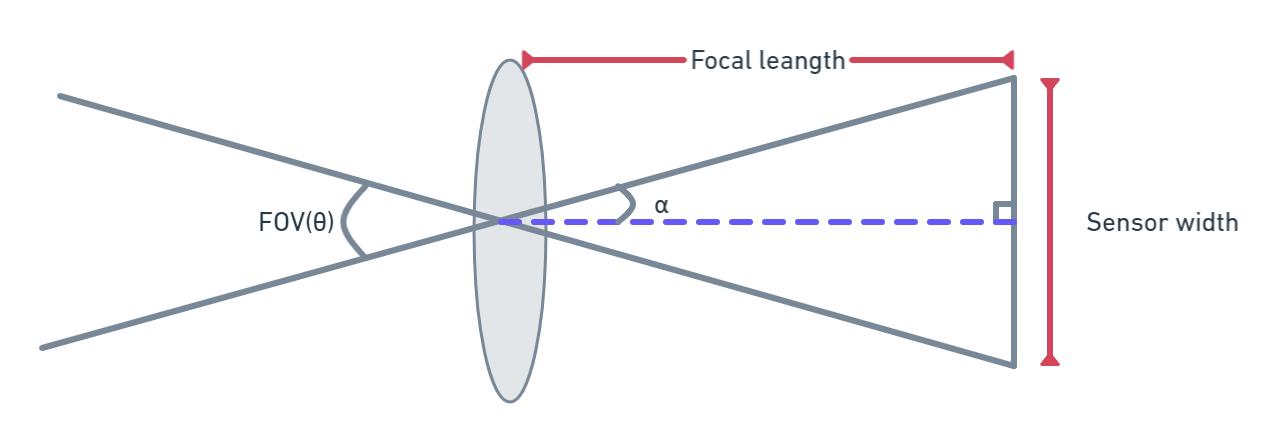
\includegraphics[width=1\textwidth]{focalLeanght.png}
        \caption{An illustration for deriving the formula for calculating field of view}
        \label{fig:focal}
    \end{figure}
    
    With equation \ref{eq:startingEQ} we can see that we need to find an expression for $\alpha$. From figure x we can derive $\alpha$ from the right angle triangle and with simple trigonometry we get the following formula:
    \begin{equation}
    \label{eq:AlphaStart}
        \frac{w}{2*f} = tan(\alpha)
    \end{equation}
    With equation \ref{eq:AlphaStart} we can now transform it to make it an expression of $\alpha$. This resuls in the following equation:
    \begin{equation}
    \label{eq:AlphaFree}
        \alpha = tan^{-1}\left(\frac{w}{2*f}\right)
    \end{equation}
    Now we can finally get an expression for $\theta$ with the help of equation \ref{eq:AlphaFree} and equation \ref{eq:startingEQ}. We get the following equation:
    \begin{equation}
    \label{eq:finalThetaEQ}
        \theta = 2*tan^{-1}\left(\frac{w}{2*f}\right)
    \end{equation}
    Equation \ref{eq:finalThetaEQ} shows the derived formula for calculating the field of view ($\theta$) as function of the focal length ($f$) and sensor width ($w$).
    \subsection*{2)  Allow two different cameras with sensor with $w_1$ and $w_2$ to have the same focal length $f$. Plot field of view $\theta_1$ and $\theta_2$ in a single graph.}
    The plot for $\theta$ as a function of $f$ for the sensor widths $w_1$ and $w_2$ is shown in figure \ref{fig:plot}.
    \begin{figure}[H]
        \centering
        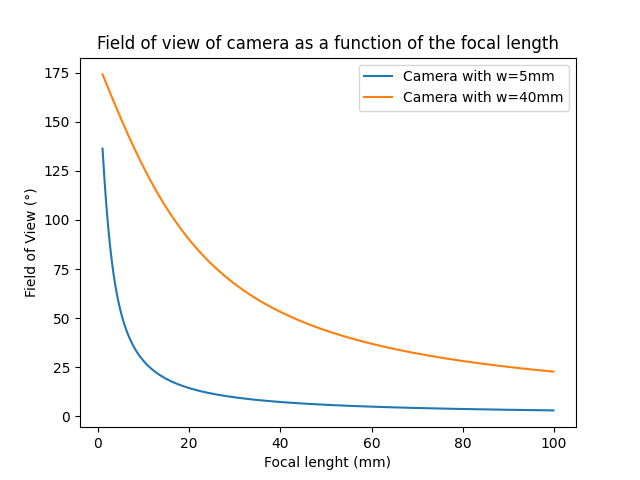
\includegraphics[width=1\textwidth]{Q2.png}
        \caption{Field of view as a function of focal length plotted with sensor width 5mm and 40mm}
        \label{fig:plot}
    \end{figure}
    \subsection*{3)  Consider two world points $x_1$ and $x_2$ and their projected 2D points $x_1^\prime$ and $x_2^\prime$ on the sensor plane. Let the points $x_1$ and $x_2$ be located in world space such that $x_1=(x, y, z)$ and $x_2=(x+dx, y, z)$. Evaluate how the distance between the projected points  $|x_2^\prime - x_1^\prime|$ varies as a function of focal lengths $f$ and depth $z$}
    Given focal length $f$ and coordinates $(x, y, z)$ we can calculate a projected 2D point with the formula from equation \ref{eq:projectionFormula}.
    \begin{equation}
        \label{eq:projectionFormula}
        \left( f\frac{x}{z}, f\frac{y}{z} \right)
    \end{equation}
    Since the only differentiating factor between $x_1$ and $x_2$ is the coordinate $x$ we can focus on that part and simplify the equation to:
    \begin{equation}
        \label{eq:SimplifiedProjectionFormula}
        |x_2^\prime - x_1^\prime| = \left| f\frac{x+dx}{z} - f\frac{x}{z} \right|
    \end{equation}
    Simplifying the expression from equation \ref{eq:SimplifiedProjectionFormula} we get the following:
    \begin{equation}
        \label{eq:finalProjection}
        |x_2^\prime - x_1^\prime| = \left| f\frac{dx}{z} \right|
    \end{equation}
    Equation \ref{eq:finalProjection} shows the final formula for calculating the distance between $x_1$ and $x_2$.
    \section{Reflections}
\end{document}